% Journal of Bioinformatics and Computational Biology submission source.
% Uses the unmodified author-supplied World Scientific class dated 2026/05/18.
\pdfminorversion=7
\pdfsuppresswarningpagegroup=1
\documentclass{ws-jbcb}
\setlength{\paperheight}{11in}

\usepackage[super]{cite}
\usepackage{xcolor}
\usepackage[verbose,hypertexnames=false]{hyperref}
\hypersetup{colorlinks=false,allbordercolors=blue,pdfborderstyle={/S/U/W 1}}
\usepackage{array}
\usepackage{tabularx}
\usepackage{xurl}

\graphicspath{{./}}

% theorem, proposition, definition, example, remark, and proof are class-native.
\newtheorem{algorithm}{Algorithm}
\numberwithin{equation}{section}

\newcommand{\tas}{\textit{Arabidopsis thaliana}}
\newcommand{\ath}{\textit{A.\ thaliana}}
\newcommand{\hs}{\textit{Homo sapiens}}
\newcommand{\TAU}{\tau}
\newcommand{\xRightarrow}[1]{\stackrel{#1}{\Longrightarrow}}
\newcommand{\LTS}{\mathcal{L}}
\newcommand{\powerset}{\mathcal{P}}
\newcommand{\strongsim}{\mathrel{\sim_{s}}}
\newcommand{\weaksim}{\mathrel{\sim_{w}}}
\newcommand{\weakpre}{\mathrel{\preceq_{w}}}
\newcolumntype{Y}{>{\raggedright\arraybackslash}X}

\hypersetup{
  pdftitle={Supplementary Validation: Locating resolution-dependent behavioral correspondence in qualitative DNA-damage response models},
  pdfauthor={Carlos Ramirez Ovalle},
  pdfkeywords={DNA-damage response, observational resolution, qualitative biological networks, model comparison, Petri nets, weak bisimulation}
}


\renewcommand{\thesection}{S\arabic{section}}
\renewcommand{\thefigure}{S\arabic{figure}}
\renewcommand{\thetable}{S\arabic{table}}
\newcommand{\DRBaseMinusEdges}{5{,}062{,}632}
\newcommand{\DRBaseMinusStates}{547{,}021}
\newcommand{\DRBasePlusEdges}{10{,}296{,}917}
\newcommand{\DRBasePlusStates}{1{,}044{,}457}
\newcommand{\DRBaseSubsetBytes}{1{,}999{,}975{,}480}
\newcommand{\DRBaseSubsetPairs}{6{,}158}
\newcommand{\DRControlMinusEdges}{21{,}544{,}296}
\newcommand{\DRControlMinusStates}{2{,}140{,}569}
\newcommand{\DRControlPlusEdges}{32{,}980{,}090}
\newcommand{\DRControlPlusStates}{3{,}133{,}393}
\newcommand{\DRDepth}{8}
\newcommand{\DRDepthStates}{73}
\newcommand{\DRFirstCommitted}{1}
\newcommand{\DRHistoryStates}{78}
\newcommand{\DRLocalBaseEdges}{2}
\newcommand{\DRLocalBaseStates}{3}
\newcommand{\DRLocalMinusEdges}{54}
\newcommand{\DRLocalMinusStates}{34}
\newcommand{\DRLocalPlusEdges}{17}
\newcommand{\DRLocalPlusStates}{12}

\begin{document}
\markboth{C. Ramirez Ovalle}{Supplementary validation for JBCB-1505}
\catchline{}{}{}{}{}
\title{Supplementary Validation: Locating resolution-dependent behavioral correspondence in qualitative DNA-damage response models}
\author{Carlos Ramirez Ovalle}
\address{Pontificia Universidad Javeriana Cali, Colombia}
\date{}
\maketitle
This supplement retains implementation-verification and exploratory-data
details supporting the main biological comparison. It includes the death-receptor execution audit in Section~S5. It is not independent wet-lab validation of either biological case.

\section{Formal and software verification}
\label{sec:computational-validation}

\subsection{Construction-level software benchmark and comparator study}
\label{sec:benchmark-method}

Six deterministic pairs were specified before any biological application. They
provide behavioral-class ground truth by construction and test whether the
software recovers intended formal distinctions; they do not provide biological
ground truth. A
12-step labeled workflow supplies identity, controlled silent subdivision, label
mismatch, label-order swap, and an added observable branch. The sixth pair is
$a.(b+c)$ versus $a.b+a.c$ from Example~1 of the main article. Table
\ref{tab:synthetic} gives construction-level and computed classes.

\begin{table}[t]
\tbl{Controlled benchmark; the expected class is not used by the classifier.
\label{tab:synthetic}}{
\begin{tabular}{@{}>{\raggedright\arraybackslash}p{0.70in}%
>{\raggedright\arraybackslash}p{1.10in}%
>{\raggedright\arraybackslash}p{1.20in}%
>{\raggedright\arraybackslash}p{1.20in}@{}}
\toprule
Case & Change & Expected & Observed \\
\colrule
Identity & exact copy & strong equivalence & strong equivalence \\
Silent refinement & insert internal steps & weak equivalence & weak equivalence \\
Label mismatch & replace an observable & not comparable & not comparable \\
Order swap & preserve counts, change order & not comparable & not comparable \\
Added branch & add an outcome & reference in candidate & reference in candidate \\
Early/late choice & move decision point & candidate in reference & candidate in reference \\
\botrule
\end{tabular}}
\end{table}

On this construction-level decision task, weak bisimulation recovered all six
binary weak-equivalence decisions. Truncated
trace equality recovered 5/6 but accepted the trace-equivalent branching pair;
LTS-GDA recovered 4/6, the structural profile 3/6, and direct PN-GDDA 2/6.
PN-GDDA assigned 1.0 to identity, silent refinement, label mismatch, and order
swap, while added-branch and branching pairs scored 0.9676 and 0.9657. No
threshold over the six PN-GDDA scores exceeded 4/6 because two negative controls
tied the positive controls at 1.0. Figure~\ref{fig:benchmark} reports all
predeclared decisions.

\begin{figure}[t]
\centering
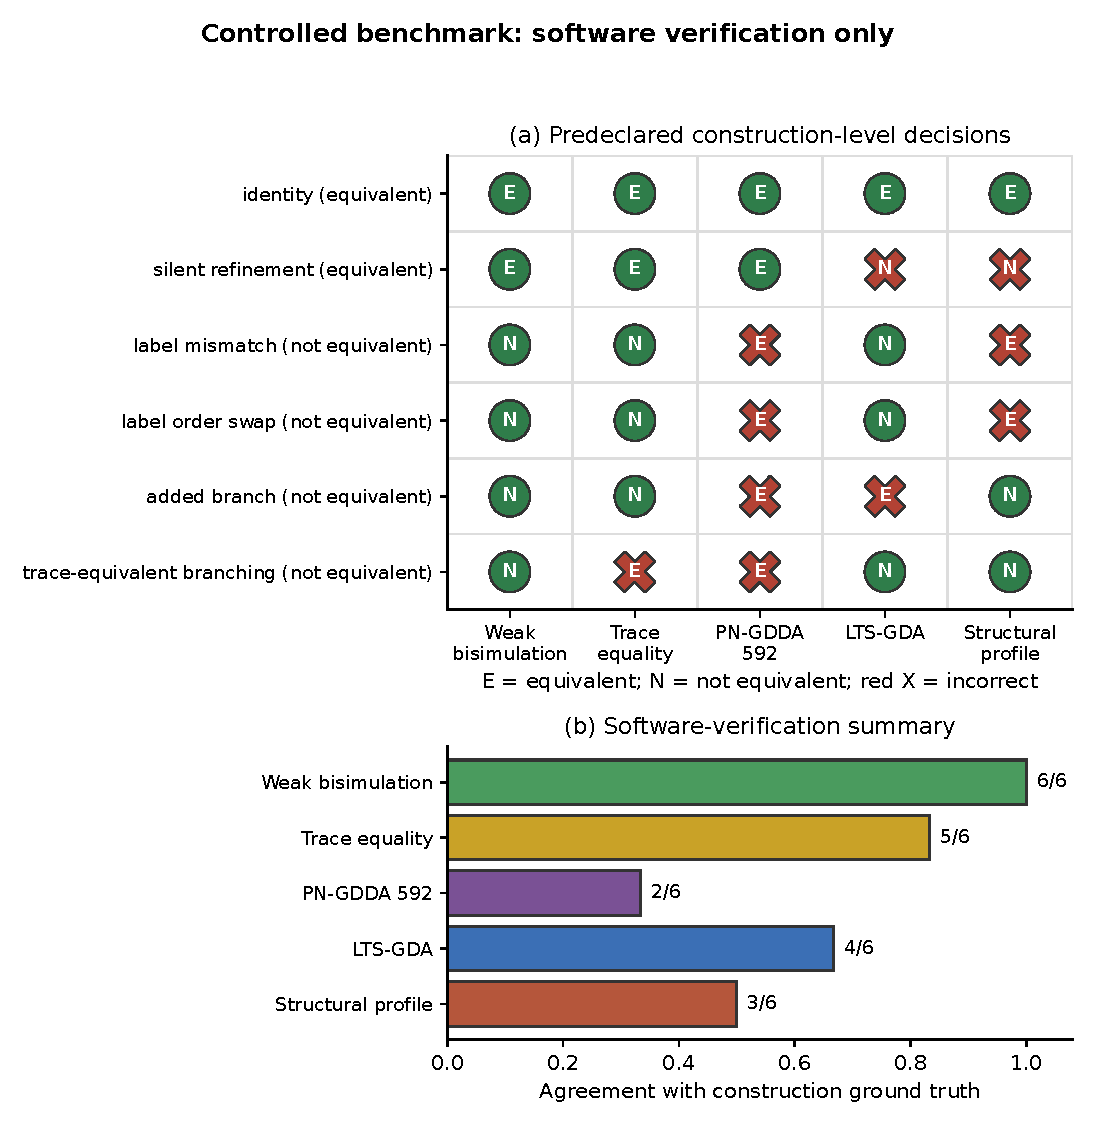
\includegraphics[width=\textwidth]{SFig1.pdf}
\caption{Controlled software/formal benchmark. (a) Decisions for six cases whose
labels were fixed by construction; a red cross marks disagreement with that
label. (b) Agreement count on this limited task. Trace equality loses branching;
PN-GDDA is label-blind; LTS-GDA retains local labels but does not abstract silent
refinement or recursively match successors. The panel verifies implementation
behavior and does not measure biological validity or generic method superiority.}
\label{fig:benchmark}
\alttext{A benchmark heatmap and bar chart comparing five methods on six
controlled model pairs.}
\end{figure}

The structural profile averages state-count, edge-count, label-multiset, and
out-degree-multiset similarities. The trace diagnostic declares a depth-$8$
match when $d_8=0$. PN-GDDA was implemented from its published definition using
151 directed bipartite graphlets and the 592 published/Holmes orbit
slots.\cite{Szawulak2022} For orbit $j$,
\begin{equation}\label{eq:pn-gdda}
N_G^j(k)=\frac{D_G^j(k)/k}{\sum_{r>0}D_G^j(r)/r},\quad
A^j(G,H)=1-\frac{\left[\sum_k(N_G^j(k)-N_H^j(k))^2\right]^{1/2}}{\sqrt{2}},
\end{equation}
and PN-GDDA is the mean $A^j$. Synthetic LTSs use an exact state-machine Petri
net encoding; curated pairs use their native nets. The 0.9 threshold is a fixed
diagnostic decision, not an equivalence relation. LTS-GDA instead combines four
reachable-graph orbits with labeled edge, two-step, divergence, and convergence
motifs.

The catalog audit recovered 151 graphlets and 592 slots from hash-verified Holmes
1.1.1/2.0.1.2 JARs. A direction- and type-preserving automorphism partition has
576 distinct orbits; using it is reported only as sensitivity. A Java probe
matched every inspected Holmes 1.1.1 topology/root assignment. On a four-node test net and
its one-arc deletion, Python and Holmes scores were 0.9872027465870733 and
0.987202746587073, agreeing to 12 decimal places. Holmes is an independent
software reference for the structural score.\cite{Radom2017}

\subsection{Independent formal oracles}\label{sec:mcrl2-method}

Each analyzed LTS was exported in Aldebaran AUT format and evaluated with
\texttt{ltscompare} from hash-pinned mCRL2 202607.0.\cite{Bunte2019} The tool
independently checked strong bisimilarity, weak bisimilarity, and exact weak-trace
equivalence with \texttt{tau} hidden. Its interface does not expose a general weak-simulation preorder. For
the tau-free Example~1 and middle strictness witness only, the audit additionally
uses its strong-simulation preorder, which coincides with weak simulation
when neither input has silent transitions; both directions agree. No such
weak-preorder claim is made for systems containing silent transitions.

A separately coded attacker--defender game grows the least set of positions from
which an unmatched move can be forced. It agreed with the production simulation
algorithm on all 67,600 ordered pairs among all 260 one- and two-state LTSs over
$\{a,\TAU\}$. This is exhaustive within that finite universe, not a proof for
arbitrary systems. Across the six synthetic pairs, six public-model controls,
and nine HPN comparisons below, Python and mCRL2 agreed on all 42 reported
strong/weak decisions. Theorem~1 of the main article, finite exhaustive testing,
and external-tool comparison are distinct evidence layers.

\subsection{Observed computational scaling and reproducibility}
\label{sec:scalability-method}

Linear workflows of 8, 16, 32, 64, 96, and 128 transitions were compared with an
identity and a silently refined copy. Median runtime over three repetitions rose
from about 0.4 ms for nine states to about 0.6 s for the largest pairs. The
128-step identity relation had 16,641 candidate pairs; refinement increased it
to 18,705 pairs over 129 and 145 states. Every class remained as constructed
(the complete plot and table are archived in the repository). Timings used
Python 3.11.8 on an Apple M3 Pro with 18 GiB memory and are machine-dependent.

The Python standard library implements reachability, formal relations, parsers,
and controlled models. NumPy, pandas, Matplotlib, NetworkX, pydot, and Graphviz
support tabulation and figures. Fixed seeds, source hashes,
machine-readable outputs, unit tests, an executed notebook, environment files,
and continuous integration are public. Runtime CSV values are excluded from
byte-level regression because they depend on hardware; all scientific outcomes
and other result tables are deterministic.

\section{Cross-format ingestion and execution controls}
\label{sec:public-method}

Two externally authored GINsim models test the complete import-to-comparison
path: the 13-component mammalian cell cycle in SBML-qual and the four-component
multilevel p53--Mdm2 model in GINML.\cite{Naldi2018,Traynard2016,
Chaouiya2013SBML,AbouJaoude2009} Files, URLs, and SHA-256 values are archived.
Unitary-asynchronous updates move one enabled component by one level and label
its direction. Each base model was compared with an exact copy, five silent
subdivisions, and a reachable-label perturbation. All six controls recovered
their predeclared strong/weak/exact-trace outcomes in Python and mCRL2
(Table~\ref{tab:public-controls}).

\begin{table}[t]
\tbl{Public GINsim models and control outcomes. S/W/T denote strong, weak, and
exact weak-trace equivalence.\label{tab:public-controls}}{
\begin{tabularx}{\textwidth}{@{}p{0.25\textwidth}lrrccc@{}}
\toprule
Model & Format & States & Edges & Copy & Silent & Perturbed \\
\colrule
Mammalian cell cycle & SBML-q & 826 & 3,413 & Y/Y/Y & N/Y/Y & N/N/N \\
p53--Mdm2 damage & GINML & 17 & 26 & Y/Y/Y & N/Y/Y & N/N/N \\
\botrule
\end{tabularx}}
\end{table}

Synchronous execution reached 13 of 826 asynchronous cell-cycle states (Jaccard
0.0157) and eight of 17 p53--Mdm2 states (Jaccard 0.471), confirming sensitivity
to update semantics. These are cross-format execution controls, not biological
validation.

\section{Exploratory HPN-DREAM/CASPOTS held-out analysis}\label{sec:hpn-method}

The public HPN-DREAM phosphoproteomic series and CASPOTS Boolean families contain
72 BT20, 191 BT549, and 21 MCF7 networks.\cite{Hill2016,Razzaq2018} One
representative per cell line was selected before test responses were read: the
model with maximum mean within-family Jaccard similarity between active clauses,
with exact lexicographic tie-breaking. This structure-only rule selected
zero-based rows 24, 137, and 9 (Table~\ref{tab:hpn-medoids}); an anti-leakage test
forbids access to test files during selection.

\begin{table}[t]
\tbl{HPN-DREAM families and structure-only representatives.
\label{tab:hpn-medoids}}{
\begin{tabular}{@{}lrrrr@{}}
\toprule
Cell line & Family & Medoid row$^a$ & Clauses & Mean Jaccard \\
\colrule
BT20  & 72  & 24  & 29 & 0.815 \\
BT549 & 191 & 137 & 25 & 0.854 \\
MCF7  & 21  & 9   & 23 & 0.851 \\
\botrule
\end{tabular}}
\begin{tabnote}$^a$Zero-based row; selected from model structure only.\end{tabnote}
\end{table}

The interface is the intersection of seven measured PI3K/MAPK/mTOR readouts.
The three common test perturbations are mTOR inhibition, IGF1 plus mTOR
inhibition, and 4EBP1 plus mTOR inhibition. Measured time-zero values initialize
readouts; stimuli and inhibitors are clamped; other relevant nodes start at zero.
Primary asynchronous LTSs label interface updates and hide all others. The nine
cross-cell pair-condition comparisons were repeated synchronously; this stress
test is not a most-permissive analysis. CASPOTS itself evaluates asynchronous
trajectories.\cite{Pauleve2020,Razzaq2018}

Experimental distance is RMSE over common post-zero times and readouts. Spearman
associations use an exact one-sided permutation of the three cell-pair labels
within each condition ($3!^3=216$). CASPOTS/Clingo compatibility scores consume
optimization to completion, use deterministic secondary tie-breaks, and were
reproduced twice. Native specificity uses the exact sign permutation of three
native-minus-mean-cross differences.

Selected LTSs had 2--44 states. None of the nine cross-cell pairs was weakly
bisimilar: six had one-way simulation and three were not comparable. Direction
was retained explicitly, with three left-model-in-right-model and three
right-model-in-left-model relations. These categories do not form a justified
one-dimensional order, and the held-out RMSE is symmetric between each cell
pair. We therefore removed the former ordinal class coding and performed no
scalar formal-class test. Descriptively, median RMSE was 0.2418 for the six
one-way relations and 0.2071 for the three non-comparable pairs; after preserving
direction, the corresponding medians were 0.2757, 0.1919, and 0.2071, each based
on only three observations. These summaries are not inferential evidence.

The two predeclared continuous diagnostics were retained. Truncated-trace
distance gave $\rho=-0.596$ (exact one-sided $p=0.556$), and LTS-GDA distance
gave $\rho=0.669$ ($p=0.097$) under 216 condition-stratified permutations.
Neither association is conclusive. Synchronous updating preserved seven of nine
formal classes.

Native medoid RMSE was 0.33024 (BT20), 0.31335 (BT549), and 0.27726 (MCF7),
against discretization RMSE 0.32944, 0.30079, and 0.27726. Native excess-RMSE
advantage over mean cross-cell medoids was 0.00212 and not established by the
exact sign test ($p=0.25$; Fig.~\ref{fig:hpn-validation}). The result demonstrates
an exploratory held-out compatibility check and separates formal similarity
from empirical response similarity; it does not demonstrate cell-line
specificity or predictive discrimination.

\begin{figure}[t]
\centering
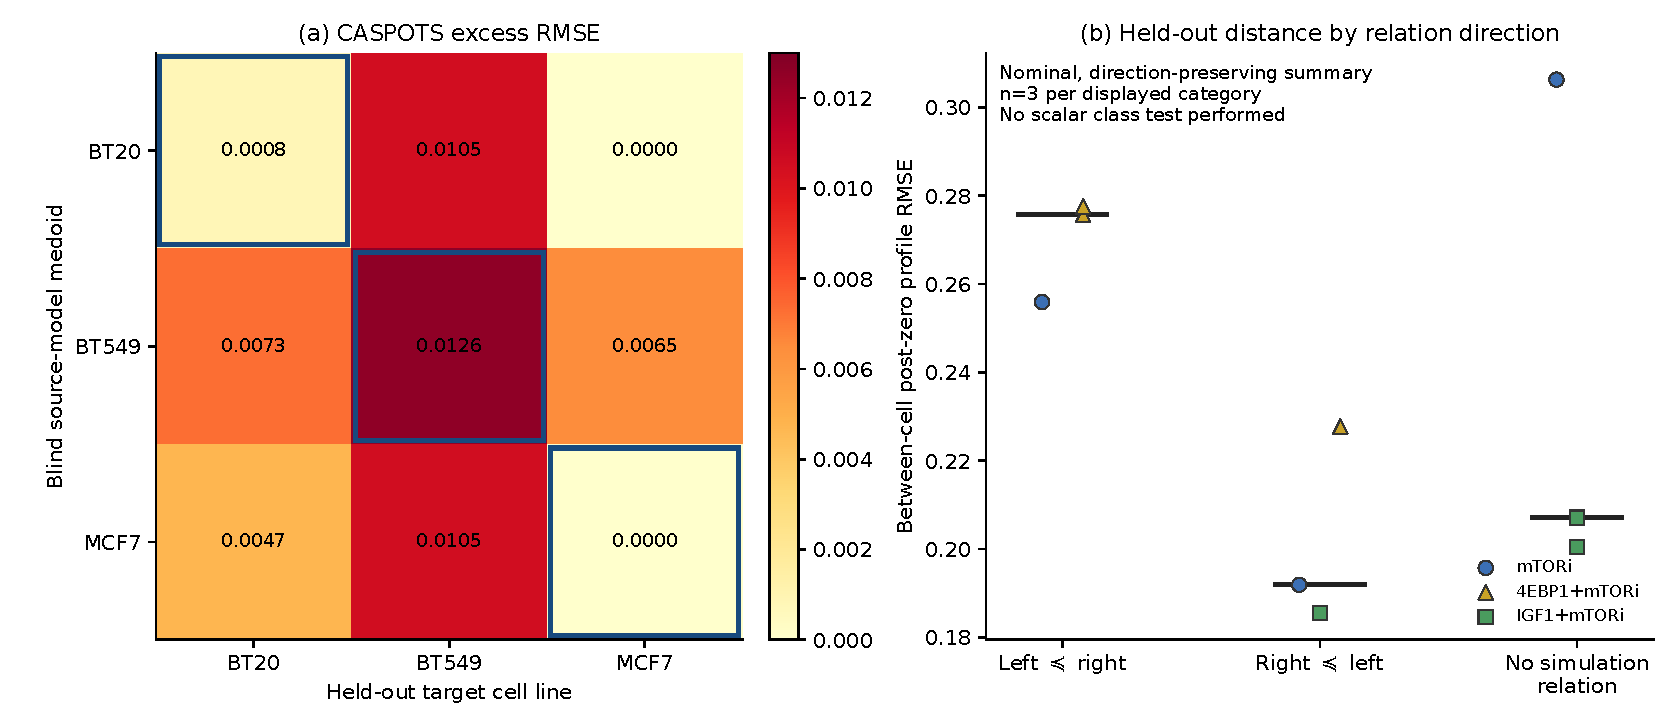
\includegraphics[width=\textwidth]{SFig2.pdf}
\caption{Exploratory held-out HPN-DREAM analysis. (a) CASPOTS excess RMSE by
source medoid and target; outlined cells are native contexts. (b) Between-cell
profile RMSE with the direction of weak simulation retained. Horizontal bars
are medians; each category has $n=3$, and no scalar formal-class test was
performed. Neither panel establishes native cell-line specificity.}
\label{fig:hpn-validation}
\alttext{CASPOTS excess-error matrix and a direction-preserving nominal display
of held-out response distances for three breast-cancer cell lines.}
\end{figure}


\section{Quantifier and direction audit}
The production implementation was not changed to conform to a proposed
reinterpretation of simulation. Instead, the audit independently constructs
silent closures and weak targets from raw edges, and grows a least losing set
in simultaneous attacker--defender rounds. It does not call the production
adjacency, closure, weak-step, or relation routines. Exact weak-trace inclusion
is checked by a finite epsilon-NFA subset-product traversal, treating all
original states as accepting, without a depth cutoff.

For Example~1 in the main article, complete acyclic path enumeration also
gives $\{\epsilon,a,ab,ac\}$ on both sides. The supplied five-pair early-to-late
relation satisfies every transfer clause. The reverse calculation first
removes $(\ell_1,e_b)$ because $c$ cannot be matched and $(\ell_1,e_c)$ because
$b$ cannot be matched; the initial pair subsequently has no surviving reply.
The machine-readable deletion certificate records these dependencies.

All three strictness witnesses and 32 ordered model pairs (six synthetic,
three GIM interfaces, five curated modules, and 18 asynchronous/synchronous
HPN comparisons) agree on strong/weak bisimilarity and both weak-simulation
directions between the production code and independent audit. Every synthetic
class still agrees with its construction-level expectation. Direction fields
explicitly state \texttt{left\_simulated\_by\_right} and
\texttt{right\_simulated\_by\_left}.

The complete one-/two-state universe contains 260 named LTSs over
$\{a,\tau\}$ with initial state zero, hence 67,600 ordered pairs. The expanded
audit found no simulation or weak-bisimulation disagreement and no failure of
the hierarchy or trace-inclusion implications. Simulation is reflexive and
transitive on this universe. There are 41,080 weakly bisimilar ordered pairs
and 4,848 mutually simulated but non-bisimilar ordered pairs. No one-way
simulation with exact trace equality occurs in this small universe; the
larger acyclic Example~1 supplies that witness. The finite enumeration
supports software correctness only; it does not replace the general proofs.

Reproduce the new audit using
\texttt{python -m src.formal\_audit} and
\texttt{python -m unittest tests.test\_formal\_audit -v}.
The four JSON/CSV reports in \texttt{results/} include the Example~1
certificate, hierarchy witnesses, all model-pair directions, and exhaustive
counts. The main article's appendix retains all definitions needed for its
claims, the relation-deletion proof, and explicit proofs of the three failed
converses. Detailed Petri nets remain in the main article rather than being
removed during compression of validation material.
\section{Death-receptor execution and witness checks}

\subsection{Provenance, initialization and reduction}
The source is the original Calzone 2010 GINsim file
\texttt{Calzone\_\_Cell\_Fate.zginml}, not the later multiscale adaptation.
Its SHA-256 is
\begin{quote}\small\ttfamily
1cdbf6a3fb00fcf7ce9d63cb753a9bf4a58\allowbreak
ea1e16486abb6a49a2016634a6993.
\end{quote}
The stored initial-state records omit input assignments. We explicitly set
TNF=FADD=ATP=cIAP=1 and all remaining nodes to zero. DR-FB- changes only the
read of CASP3 within the CASP8 rule, preserving CASP3's own rule and every
other component. All 16 combinations of the four CASP8 regulators are tested
against the declared original and edge-deletion truth tables.

The original prospective configuration and two dated resource amendments are
retained without overwriting their history. The first object-based execution
exceeded 200,000 states; the hidden-sink quotient also exceeded that limit and
a diagnostic one-million-state limit. These runs produced no formal relation
decision. Compact Boolean enumeration then completed all four reachable
graphs. The 28-node source has three fixed inputs in the sustained protocol
and three omitted hidden sinks; withdrawal makes TNF dynamic. The retained
universe is therefore bounded by $2^{22}$ and $2^{23}$ Boolean valuations,
respectively, before reachability restriction.

Removal of NonACD, Apoptosis and Survival is not the source paper's reduced
conceptual model. These three output nodes regulate no retained component and
are not in the fixed interface. Relating states with identical retained
coordinates gives a weak bisimulation: output updates are matched by zero
silent steps, and retained updates have identical enabling conditions and
successors in both directions. Output values can independently settle at a
terminal retained state. Terminal classification uses NFkB/CASP3/MPT and ATP,
not the omitted delayed output copies. Strong relations are not inferred from
this weak reduction. The selected full 28-node continuations are also checked
directly against their quotients and reproduce the reported weak relations.

\subsection{Exact checks, limits and distinct comparison scopes}

The sustained graphs contain \DRBasePlusStates{} and \DRBaseMinusStates{}
states, with \DRBasePlusEdges{} and \DRBaseMinusEdges{} edges. The withdrawal
graphs contain \DRControlPlusStates{} and \DRControlMinusStates{} states,
with \DRControlPlusEdges{} and \DRControlMinusEdges{} edges. All reachable
terminal components are singleton fixed points. This is enumeration of
possibilities, not a reproduction of Monte Carlo phenotype probabilities or
physical-time calibration in the original publication.

The exact epsilon-NFA subset-product search accepts every nonempty state
subset and rejects only the empty subset, thereby checking prefix-closed
finite weak languages without a depth cutoff. The original limits of 10,000
subset pairs, 250,000,000 stored bytes and 180 seconds did not decide the
sustained comparison. A subsequent resource amendment increased only its
search limits to 100,000 pairs, 2,000,000,000 bytes and 600 seconds. It reached
\DRBaseSubsetPairs{} pairs and \DRBaseSubsetBytes{} stored bytes before the
memory cap, after finding this DR-FB+-only 12-action word:
\begin{quote}\small\raggedright
MPT\_up, CASP3\_up, CASP3\_down,\\
NFkB\_up, NFkB\_down, MPT\_down,\\
CASP3\_up, CASP3\_down, CASP3\_up,\\
CASP3\_down, CASP3\_up, CASP3\_down.
\end{quote}
The complete subset search remains unfinished, but this finite counterexample
refutes global sustained trace equality. The reverse inclusion remains
undecided. The reproducible driver rechecks the word explicitly, even if a
later discovery search hits a resource cap sooner.

Independent SciPy directed reachability gives 8,264, 7,936 and 8,064 accepting
states for the last three prefixes in DR-FB+, versus 744, 120 and zero in
DR-FB-. A reconstructed 53-update positive path satisfies the original
28-node rule callbacks. Independent mCRL2 antichain checks include the word's
finite prefix-language in DR-FB+ but not in DR-FB-, using a 180-second limit
per command. The negative sparse check uses the proven hidden-sink projection;
it is not a direct exhaustive search of the full 28-node product. The latter
reached a 100,000-state cap for both variants and remains inconclusive.
These distinctions prevent a partial audit from being presented as a proof.

The failed sustained inclusion also refutes the corresponding weak simulation
and weak bisimulation, without completing a global relation game. Direct
global games exceed their one-million-pair budget. Earlier full-graph external
checks had 180-second limits, and an additional global antichain inclusion
check reached 600 seconds without a decision. None of these timeouts is the
basis of the inequality result. Withdrawal search retains its original limits.

The withdrawal search instead finds exact counterexamples in both directions:
\begin{quote}\small
DR-FB+ only: withdraw\_TNF, CASP3\_up, CASP3\_down, CASP3\_up.\\
DR-FB- only: CASP3\_up, withdraw\_TNF, CASP3\_down.
\end{quote}
For each word, epsilon-closure propagation leaves a nonempty accepting subset
in one system and an empty subset in the other. Once both inclusions are
refuted, exhaustive exploration of every other word is unnecessary. Weak
simulation would imply the corresponding trace inclusion, so both global weak
simulations, and therefore both bisimilarities, fail for the intervention
protocol. This inference is from exact counterexamples, not from a timeout or
from the state-specific continuation certificate.

A second implementation checks these two words using a direct product of the
original 28-node tuple states and word positions. It does not use compact
truth tables, projected graphs, or the sink reduction. For the DR-FB+-only
word it finds an accepting execution in DR-FB+ (5,356 visited product states)
and exhausts DR-FB- (3,747 states) without acceptance. For the DR-FB--only word
it exhausts DR-FB+ (929 states) and finds acceptance in DR-FB- (1,124 states).
Thus both global counterexamples are independently confirmed in the full
source-rule models.

The automatically selected shared state occurs after eight raw updates. Its
sustained continuations are three-state/two-edge silent graphs, with exact
language $\{\epsilon\}$. Allowing withdrawal yields 12-state/17-edge and
34-state/54-edge graphs. Exact subset-product exploration has four reachable
subset pairs. The positive continuation is simulated by the negative one;
the reverse fails. The deletion certificate begins at their initial pair and
retains every possible weak defending reply, with strictly smaller deletion
ranks at dependencies. Independent verification reconstructs these replies
from the raw edges, and rejects a deliberately truncated certificate in the
unit tests. mCRL2 agrees on strong/weak bisimilarity and exact weak traces for
both sustained and intervention-conditioned comparisons. Its arbitrary
weak-simulation preorder is not assumed to be available.

\subsection{History aggregation and the event-depth scan}

The common raw path is TNFR, DISC\_TNF, CASP8, BAX, MOMP, Cyt\_c,
apoptosome, CASP3 activation, in that order. Its visible projection contains
only CASP3 activation. Exact closure propagation shows 78 hidden states in
each model compatible with that visible history. Their aggregated terminal
futures after immediate withdrawal are apoptosis/naive/necrosis for DR-FB+
and naive/necrosis for DR-FB-. The selected retained state is therefore not
claimed to be uniquely identified by the visible prefix.

The scan propagates all states reachable after exactly $k$ raw component
updates, for $k=0,\ldots,40$. It then applies the same single TNF withdrawal
and reads complete terminal-future sets from the fully enumerated controlled
graph. There is no future-depth truncation. Terminal states are not padded
with fictitious updates. At depth eight, one of 73 states in DR-FB+ has both
unique apoptotic terminal fate and persistent CASP3 after withdrawal. No
earlier depth has such a state. The reported counts weight states equally
only as counts, not as trajectories or cell probabilities. The scan does not
assert that no later behavior exists beyond depth 40; the entire reachable
graph and the selected witness are analyzed separately.

The naive signature is a logical readout combination, not evidence of cellular
rescue after irreversible apoptosis. A joint marker assay after withdrawal
would test a model-derived prediction; cell type, physical timing, selective
edge manipulation and wet-lab confirmation remain outside this study.

\begin{thebibliography}{10}
\providecommand{\url}[1]{\texttt{#1}}
\providecommand{\urlprefix}{URL }
\expandafter\ifx\csname urlstyle\endcsname\relax
  \providecommand{\doi}[1]{doi:\discretionary{}{}{}#1}\else
  \providecommand{\doi}{doi:\discretionary{}{}{}\begingroup
  \urlstyle{rm}\Url}\fi

\bibitem{Szawulak2022}
Szawulak B, Formanowicz P, Graphlets in comparison of {Petri} net-based models
  of biological systems, \emph{Scientific Reports} \textbf{12}:20942, 2022.
\newblock \doi{10.1038/s41598-022-24535-5}.

\bibitem{Radom2017}
Radom M, Rybarczyk A, Szawulak B, Andrzejewski H, Chabelski P, Kozak A,
  Formanowicz P, Holmes: A graphical tool for development, simulation and
  analysis of {Petri} net based models of complex biological systems,
  \emph{Bioinformatics} \textbf{33}(23):3822--3823, 2017.
\newblock \doi{10.1093/bioinformatics/btx492}.

\bibitem{Bunte2019}
Bunte O, Groote JF, Keiren JJA, Laveaux M, Neele T, de~Vink EP, Wesselink W,
  Wijs A, Willemse TAC, The {mCRL2} toolset for analysing concurrent systems:
  Improvements in expressivity and usability,  \emph{Tools and Algorithms for
  the Construction and Analysis of Systems (TACAS 2019)}, Lecture Notes in
  Computer Science, Vol.~11428, Springer, pp. 21--39, 2019.
\newblock \doi{10.1007/978-3-030-17465-1_2}.

\bibitem{Naldi2018}
Naldi A, Hernandez C, Abou-Jaoud\'e W, Monteiro PT, Chaouiya C, Thieffry D,
  Logical modeling and analysis of cellular regulatory networks with {GINsim}
  3.0, \emph{Frontiers in Physiology} \textbf{9}:646, 2018.
\newblock \doi{10.3389/fphys.2018.00646}.

\bibitem{Traynard2016}
Traynard P, Faur\'e A, Fages F, Thieffry D, Logical model specification aided
  by model-checking techniques: Application to the mammalian cell cycle
  regulation, \emph{Bioinformatics} \textbf{32}(17):i772--i780, 2016.
\newblock \doi{10.1093/bioinformatics/btw457}.

\bibitem{Chaouiya2013SBML}
Chaouiya C, B\'erenguier D, Keating SM, Naldi A, van Iersel MP, Rodriguez N,
  \emph{et~al.}, {SBML} qualitative models: a model representation format and
  infrastructure to foster interactions between qualitative modelling
  formalisms and tools, \emph{BMC Systems Biology} \textbf{7}:135, 2013.
\newblock \doi{10.1186/1752-0509-7-135}.

\bibitem{AbouJaoude2009}
Abou-Jaoud\'e W, Ouattara DA, Kaufman M, From structure to dynamics: Frequency
  tuning in the p53--mdm2 network, \emph{Journal of Theoretical Biology}
  \textbf{258}(4):561--577, 2009.
\newblock \doi{10.1016/j.jtbi.2009.02.005}.

\bibitem{Hill2016}
Hill SM, Heiser LM, Cokelaer T, Unger M, Nesser NK, Carlin DE, \emph{et~al.},
  Inferring causal molecular networks: Empirical assessment through a
  community-based effort, \emph{Nature Methods} \textbf{13}(4):310--318, 2016.
\newblock \doi{10.1038/nmeth.3773}.

\bibitem{Razzaq2018}
Razzaq M, Paulev{\'e} L, Siegel A, Saez-Rodriguez J, Bourdon J, Guziolowski C,
  Computational discovery of dynamic cell line specific boolean networks from
  multiplex time-course data, \emph{PLOS Computational Biology}
  \textbf{14}(10):e1006538, 2018.
\newblock \doi{10.1371/journal.pcbi.1006538}.

\bibitem{Pauleve2020}
Paulev{\'e} L, Kol{\v{c}}{\'a}k J, Chatain T, Haar S, Reconciling qualitative,
  abstract, and scalable modeling of biological networks, \emph{Nature
  Communications} \textbf{11}:4256, 2020.
\newblock \doi{10.1038/s41467-020-18112-5}.

\end{thebibliography}

\end{document}
